\documentclass{standalone}
\usepackage{tikz}

\begin{document}
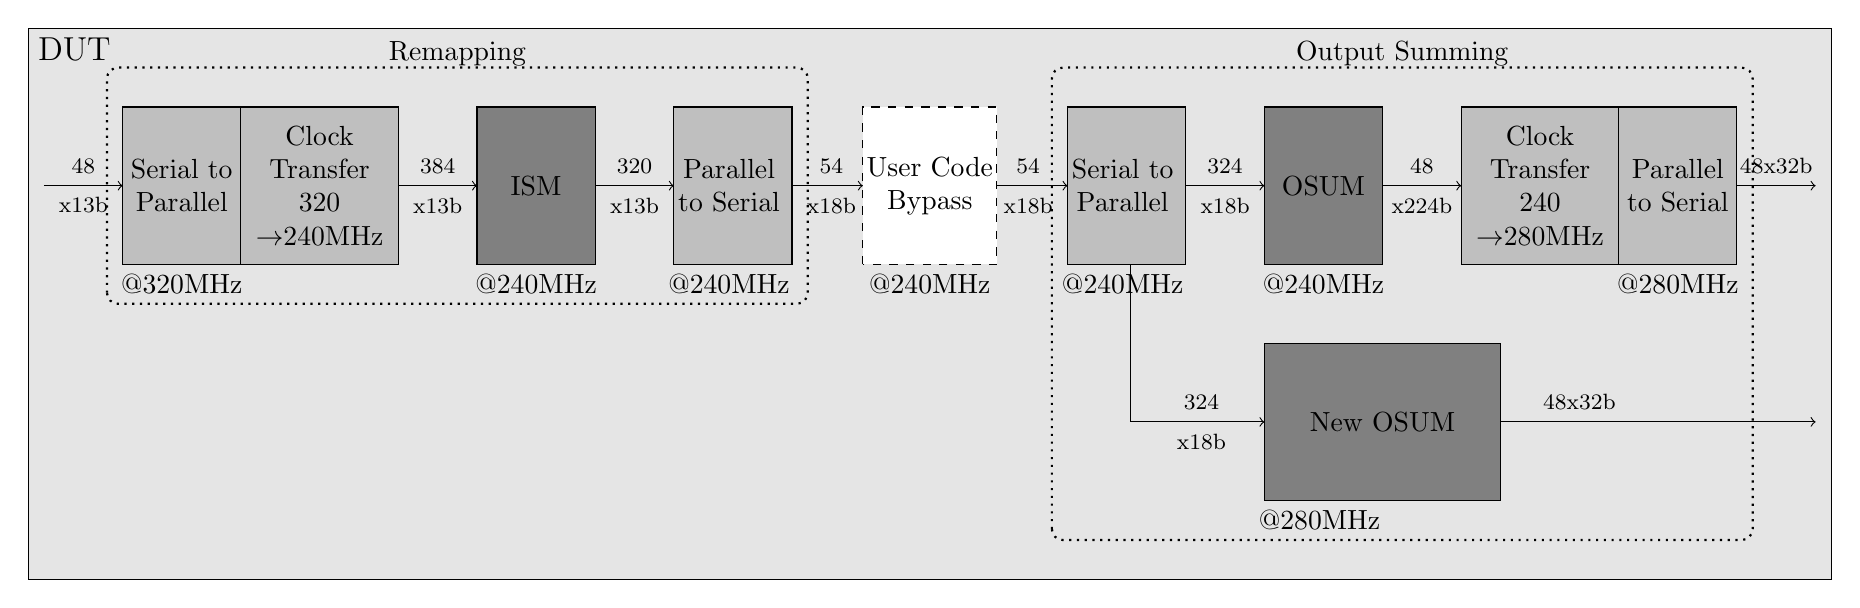
\begin{tikzpicture}[]

    % Background rectangle with borders (larger)
    \draw[fill=gray!20] (-1.2,-4) rectangle (21.7,3);
    
    % "DUT" at the top left of the background rectangle
    \node[anchor=north west, font=\large] at (-1.2,3) {DUT};
    
    % 1st block: Serial to Parallel Conversion / Clock Transfer 320MHz -> 240MHz (light gray)
    \draw[fill=lightgray] (0,0) rectangle (3.5,2);
    \draw (1.5,0) -- (1.5,2);
    \node[align=center] at (0.75,1) {Serial to \\ Parallel};
    \node[align=center] at (2.5,1) {Clock \\ Transfer \\ 320 \\ $\rightarrow$240MHz};
    \node[align=right] at (0.75,-0.25) {@320MHz};
    
    % Arrow coming into the 1st block
    \draw[->] (-1,1) -- (0,1);
    \node at (-0.5,1.25) {\footnotesize 48};
    \node at (-0.5,0.755) {\footnotesize x13b};
    
    % Arrow coming out of the 1st block
    \draw[->] (3.5,1) -- (4.5,1);
    \node at (4,1.25) {\footnotesize 384};
    \node at (4,0.75) {\footnotesize x13b};
    
    % 2nd block: ISM (dark gray)
    \draw[fill=gray] (4.5,0) rectangle (6,2);
    \node at (5.25,1) {ISM};
    \node[align=right] at (5.25,-0.25) {@240MHz};
    
    % Arrow coming out of the 2nd block
    \draw[->] (6,1) -- (7,1);
    \node at (6.5,1.25) {\footnotesize 320};
    \node at (6.5,0.75) {\footnotesize x13b};
    
    % 3rd block: Parallel to Serial Conversion (light gray)
    \draw[fill=lightgray] (7,0) rectangle (8.5,2);
    \node[align=center] at (7.7,1) {Parallel \\ to Serial};
    \node[align=right] at (7.7,-0.25) {@240MHz};
    
    % Arrow coming out of the 3rd block
    \draw[->] (8.5,1) -- (9.4,1);
    \node at (9,1.25) {\footnotesize 54};
    \node at (9,0.75) {\footnotesize x18b};
    
    % 4th block: User Code Bypass (dashed border)
    \draw[dashed, fill=white] (9.4,0) rectangle (11.1,2);
    \node[align=center] at (10.25,1) {User Code \\ Bypass};
    \node[align=right] at (10.25,-0.25) {@240MHz};
    
    % Arrow coming out of the 4th block
    \draw[->] (11.1,1) -- (12,1);
    \node at (11.5,1.25) {\footnotesize 54};
    \node at (11.5,0.75) {\footnotesize x18b};
    
    % 5th block: Serial to Parallel Conversion (light gray)
    \draw[fill=lightgray] (12,0) rectangle (13.5,2);
    \node[align=center] at (12.7,1) {Serial to \\ Parallel};
    \node[align=right] at (12.7,-0.25) {@240MHz};
    
    % Arrow coming out of the 5th block
    \draw[->] (13.5,1) -- (14.5,1);
    \node at (14,1.25) {\footnotesize 324};
    \node at (14,0.75) {\footnotesize x18b};
    
    % 6th block: OSUM (dark gray)
    \draw[fill=gray] (14.5,0) rectangle (16,2);
    \node at (15.25,1) {OSUM};
    \node[align=right] at (15.25,-0.25) {@240MHz};
    
    % Arrow coming out of the 6th block
    \draw[->] (16,1) -- (17,1);
    \node at (16.5,1.25) {\footnotesize 48};
    \node at (16.5,0.75) {\footnotesize x224b};
    
    % 7th block: Parallel to Serial Conversion / Clock Transfer 240MHz -> 280MHz
    \draw[fill=lightgray] (17,0) rectangle (20.5,2);
    \draw (19,0) -- (19,2);
    \node[align=center] at (18,1) {Clock \\ Transfer \\ 240 \\ $\rightarrow$280MHz};
    \node[align=center] at (19.75,1) {Parallel \\ to Serial};
    \node[align=right] at (19.75,-0.25) {@280MHz};
    
    % Arrow coming out of the 7th block
    \draw[->] (20.5,1) -- (21.5,1);
    \node at (21,1.25) {\footnotesize 48x32b};
    
    % New OSUM block (larger, dark gray)
    \draw[fill=gray] (14.5,-3) rectangle (17.5,-1);
    \node at (16,-2) {New OSUM};
    \node[align=right] at (15.2,-3.25) {@280MHz};
    
    % Right-angle arrow connecting Serial to Parallel Conversion to New OSUM
    \draw[->] (12.8,0) -- (12.8,-2) -- (14.5,-2);
    \node at (13.7,-1.75) {\footnotesize 324};
    \node at (13.7,-2.25) {\footnotesize x18b};
    
    % Arrow coming out of New OSUM to the right
    \draw[->] (17.5,-2) -- (21.5,-2);
    \node at (18.5,-1.75) {\footnotesize 48x32b};
    
    % Remapping rectangle (dotted border, rounded corners)
    \draw[rounded corners, dotted, thick] (-0.2,-0.5) rectangle (8.7,2.5);
    \node[anchor=south] at (4.25,2.4) {Remapping};
    
    % Output Summing rectangle (dotted border, rounded corners)
    \draw[rounded corners, dotted, thick] (11.8,-3.5) rectangle (20.7,2.5);
    \node[anchor=south] at (16.25,2.4) {Output Summing};
    
\end{tikzpicture}
\end{document}